%texexptitled======================================================================
% lab1-gcd
%-----------------------------------------------------------------------
%

\documentclass[11pt]{article}

% Package includes

\usepackage{graphicx}
\usepackage{color}
\usepackage{comment}
\usepackage{multirow}
\usepackage{askmaps}
\usepackage{amssymb}
\usepackage{amsmath}
\usepackage{tikz}
\usepackage{circuitikzgit}
\usetikzlibrary{arrows, positioning, shapes.geometric, circuits.logic.US}
\tikzstyle{line}=[draw]
\tikzstyle{arrow}=[draw, -latex]

% Wrap long URLs with hyphens
\PassOptionsToPackage{hyphens}{url}\usepackage{hyperref}
\usepackage{pdftexcmds}
\usepackage{upquote}
\usepackage{textcomp}
\usepackage{minted}
\usepackage[listings]{tcolorbox}
\usepackage{enumerate}
\usepackage{enumitem}
\usepackage{mathtools}
\DeclarePairedDelimiter{\ceil}{\Big\lceil}{\Big\rceil}

\tcbset{
texexp/.style={colframe=black, colback=lightgray!15,
         coltitle=white,
         fonttitle=\small\sffamily\bfseries, fontupper=\small, fontlower=\small},
     example/.style 2 args={texexp,
title={Question \thetcbcounter: #1},label={#2}},
}

\newtcolorbox{texexp}[1]{texexp}
\newtcolorbox[auto counter]{texexptitled}[3][]{%
example={#2}{#3},#1}

\setlength{\topmargin}{-0.5in}
\setlength{\textheight}{9in}
\setlength{\oddsidemargin}{0in}
\setlength{\evensidemargin}{0in}
\setlength{\textwidth}{6.5in}

% Useful macros

\newcommand{\note}[1]{{\bf [ NOTE: #1 ]}}
\newcommand{\fixme}[1]{{\bf [ FIXME: #1 ]}}
\newcommand{\wunits}[2]{\mbox{#1\,#2}}
\newcommand{\um}{\mbox{$\mu$m}}
\newcommand{\xum}[1]{\wunits{#1}{\um}}
\newcommand{\by}[2]{\mbox{#1$\times$#2}}
\newcommand{\byby}[3]{\mbox{#1$\times$#2$\times$#3}}


\newenvironment{tightlist}
{\begin{itemize}
 \setlength{\parsep}{0pt}
 \setlength{\itemsep}{-2pt}}
{\end{itemize}}

\newenvironment{titledtightlist}[1]
{\noindent
 ~~\textbf{#1}
 \begin{itemize}
 \setlength{\parsep}{0pt}
 \setlength{\itemsep}{-2pt}}
{\end{itemize}}

% Change spacing before and after section headers

\makeatletter
\renewcommand{\section}
{\@startsection {section}{1}{0pt}
 {-2ex}
 {1ex}
 {\bfseries\Large}}
\makeatother

\makeatletter
\renewcommand{\subsection}
{\@startsection {subsection}{1}{0pt}
 {-1ex}
 {0.5ex}
 {\bfseries\normalsize}}
\makeatother

% Reduce likelihood of a single line at the top/bottom of page

\clubpenalty=2000
\widowpenalty=2000

% Other commands and parameters

\pagestyle{myheadings}
\setlength{\parindent}{0in}
\setlength{\parskip}{10pt}

% Commands for register format figures.

\newcommand{\instbit}[1]{\mbox{\scriptsize #1}}
\newcommand{\instbitrange}[2]{\instbit{#1} \hfill \instbit{#2}}

\graphicspath{{./figs/}}


%-----------------------------------------------------------------------
% Document
%-----------------------------------------------------------------------

\begin{document}
\def\PYZsq{\textquotesingle}

\renewcommand{\arraystretch}{1.5}

\newcommand{\headertext}{EE240B HW 2}
\renewcommand{\thesubsection}{\thesection.\alph{subsection}}

\newcommand{\Ohms}{\text{ }\Omega}
\newcommand{\MOhms}{\text{ M}\Omega}

\newcommand{\nVNoise}{\frac{\text{nV}}{\sqrt{\text{Hz}}}}

\title{\vspace{-0.4in}\Large \bf \headertext \vspace{-0.1in}}
\author{Vighnesh Iyer}

\date{\today}
\maketitle

\markboth{\headertext}{\headertext}
\thispagestyle{empty}

\section{Electronic Noise}
\begin{figure}[H]
  \centering
  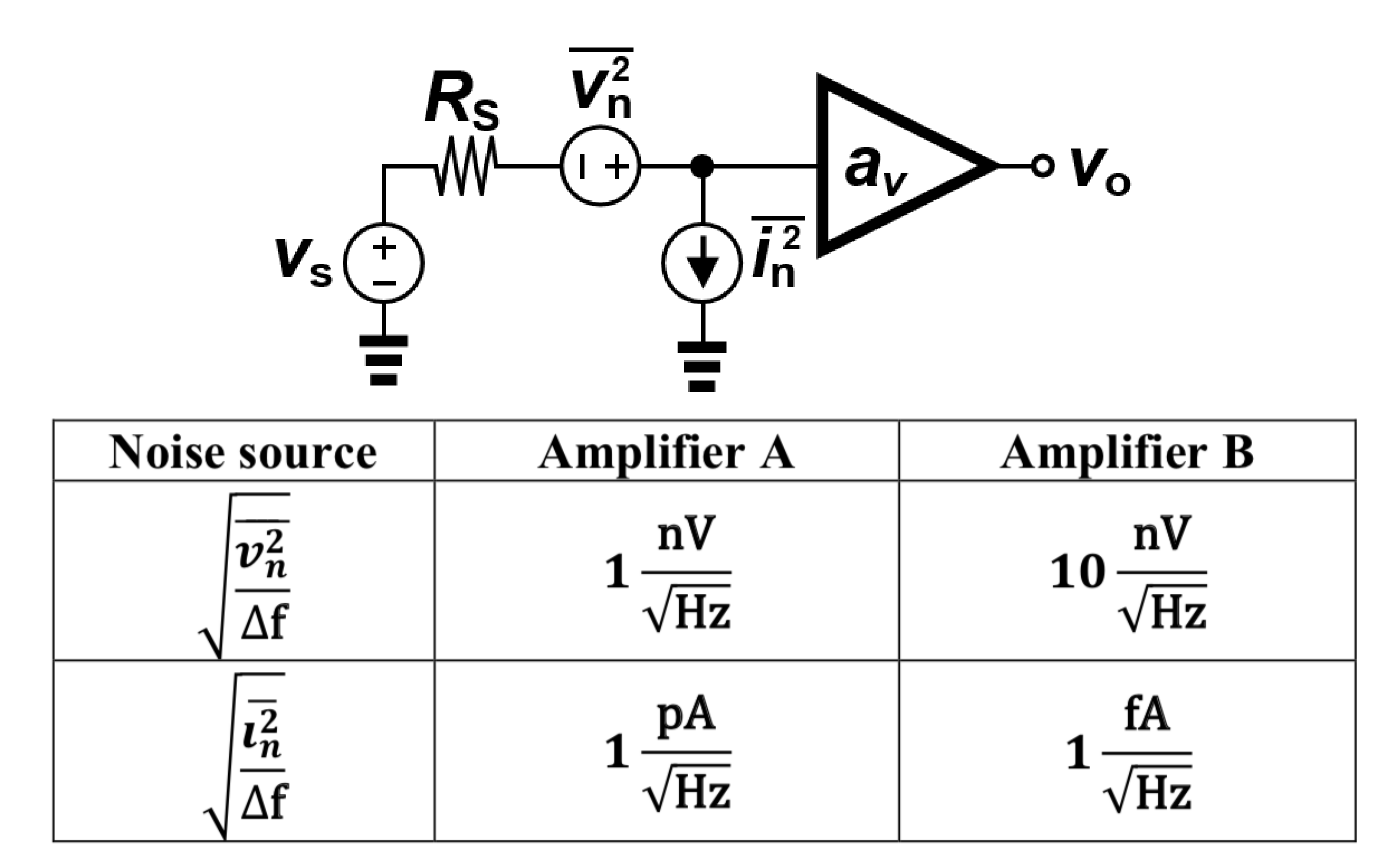
\includegraphics[width=0.5\textwidth]{figs/problem1.png}
\end{figure}

\begin{enumerate}[label=(\alph*)]
  \item {\color{blue}Calculate the input referred noise in $V / \sqrt{\text{Hz}}$ achieved with the two amplifiers for $R_S = 50 \Omega, 5 \text{M}\Omega$. Only consider the amplifier noise. Assume the amplifier voltage and current sources are uncorrelated.}

  \begin{center}
    \begin{tabular}{ |c|c|c| }
      \hline
      $R_s$ & Amplifier A & Amplifier B \\ \hline
      $50 \Ohms$ & $1.05 \nVNoise$ & $10 \nVNoise$ \\ \hline
      $5 \MOhms$ & $5000 \nVNoise$ & $15 \nVNoise$ \\ \hline
    \end{tabular}
  \end{center}

  \item {\color{blue}Significance of the result?}

  If the input voltage source's resistance is low, an amplifier with low voltage noise should be chosen (since the amplifier's current noise won't see a large resistance). Use a BJT op-amp.

  If the input voltage source's resistance is high, an amplifier with low current noise should be chosen. This is usually a FET op-amp.
\end{enumerate}

\section{Amplifier Noise}
Derive analytical expressions as a function of $g_m, \gamma, f_T, R_L, R_S,$ and $C_L$
\begin{figure}[H]
  \centering
  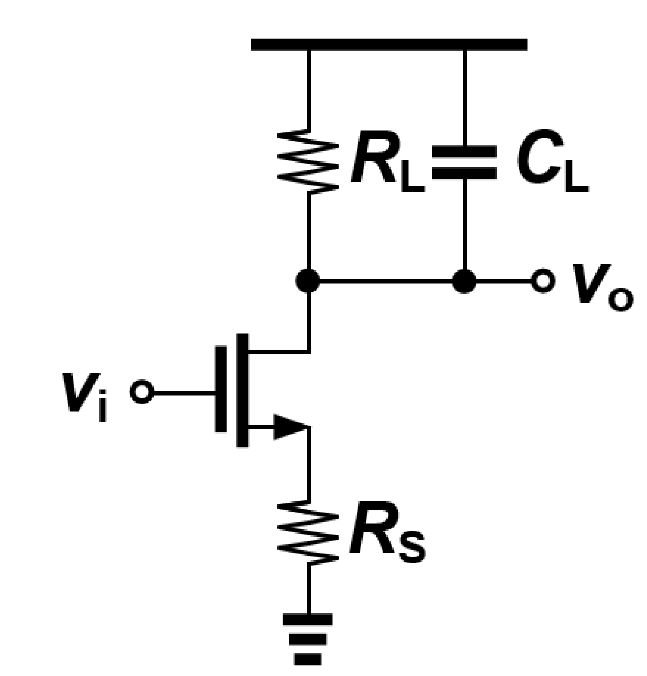
\includegraphics[width=0.2\textwidth]{figs/problem2.png}
\end{figure}

\begin{enumerate}[label=(\alph*)]
  \item {\color{blue}The voltage gain $a_v(s) = v_o / v_i$}

    This is a standard source-degenerated common-source amplifier with a complex load.
    \begin{align*}
      Z_L = (R_L || C_L) = (R_L || \frac{1}{s C_L}) &= \frac{R_L}{a + s R_L C_L} \\
      a_v(s) &= 
    \end{align*}
\end{enumerate}
\end{document}
